\section{中国剩余定理}
\label{sec:04-Discrete-Mathematics/04-Number-Theory/04}

《孙子算经》里有一道题：一堆东西，三个三个数余二，五个五个数余三，七个七个数余二，问总数几何。答案是 23。

三次清点各自只看到局部信息，谁也说不出总数，合在一起却把 0 到 104 之间的整数锁定到唯一一个。这件事比它的年纪要现代得多。把``总数''换成一个大整数上的计算，把三次清点换成三台机器分别在小模数下算自己那份，问题就成了：局部结果能不能无损地拼回全局？答案取决于模数之间的关系，而条件出人意料地简单。

上一节压缩的是指数，这一节压缩模数本身。

\begin{center}
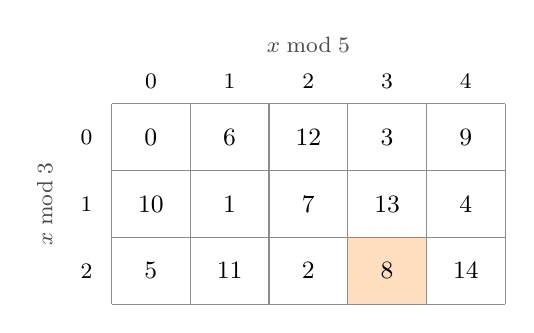
\begin{tikzpicture}[x=1cm,y=1cm,font=\small]
  \fill[orange!25] (3,0) rectangle (4,0.85);
  \draw[black!45] (0,0) grid[xstep=1,ystep=0.85] (5,2.55);
  \foreach \i/\j/\v in {0/0/0, 0/1/6, 0/2/12, 0/3/3, 0/4/9,
                        1/0/10, 1/1/1, 1/2/7, 1/3/13, 1/4/4,
                        2/0/5, 2/1/11, 2/2/2, 2/3/8, 2/4/14}{
    \node at ({\j+0.5},{2.125-0.85*\i}) {\(\v\)};}
  \foreach \i in {0,1,2}{\node[left,font=\footnotesize] at (-0.12,{2.125-0.85*\i}) {\(\i\)};}
  \foreach \j in {0,...,4}{\node[above,font=\footnotesize] at ({\j+0.5},2.62) {\(\j\)};}
  \node[font=\footnotesize,black!70] at (2.5,3.3) {\(x\bmod 5\)};
  \node[rotate=90,font=\footnotesize,black!70] at (-0.85,1.275) {\(x\bmod 3\)};
\end{tikzpicture}

\emph{模 15 的十五个余数类与 \(3\times5\) 的格点一一对应，每格恰好坐一个数。高亮格所在的行列是 \(x\equiv2\pmod3\)、\(x\equiv3\pmod5\)，从图上直接读出 \(x\equiv8\pmod{15}\)。加一在网格里是往右下角斜走一步（越界即绕回），走满十五步才回到左上角——正是 3 与 5 互素的效果。}
\end{center}

\subsection{格子不重不漏，靠的是互素}

图上没有空格也没有两个数挤在一起，这两件事各有理由，而且都短。

不漏是计数：模 15 有十五个余数类，格点也是十五个，只要证明没有碰撞，鸽巢原理反过来用就补齐了满射。不重则要动用互素。若两个整数落在同一格，它们的差同时被 3 和 5 整除；\(3\mid t\) 意味着 \(t=3s\)，代入 \(5\mid 3s\)，而 \(\gcd(5,3)=1\)，由上一节反复用过的那条推理得 \(5\mid s\)，于是 \(15\mid t\)，两个数在模 15 下本来就是同一个。互素在这里挡住的是重复计数：若模数换成 3 与 6，差被两者整除只保证被 6 整除，而不是被 18 整除，格子就会撞在一起。

\begin{theorem}[中国剩余定理]
设 \(n_1,\dots,n_k\) 两两互素，\(N=n_1\cdots n_k\)。则对任意给定的 \(a_1,\dots,a_k\)，同余方程组 \(x\equiv a_i\pmod{n_i}\)（\(i=1,\dots,k\)）有解，且解在模 \(N\) 下唯一。
\end{theorem}

论证与上面两段一字不差，只需把 3 和 5 换成一般的 \(n_i\)。注意存在性是数出来的，不是构造出来的：先知道对应是单射，再由两边个数相同断定它是双射，于是每一组余数都被某个 \(x\) 取到。

\subsection{构造：让每一项只在一个模下发声}

要真把 \(x\) 写出来，办法是造一组``开关''。记 \(N_i=N/n_i\)，它含有除 \(n_i\) 外的全部因子，因而与 \(n_i\) 互素，模逆存在。取 \(M_i\) 满足 \(N_iM_i\equiv1\pmod{n_i}\)，令

\[
x=\sum_{i=1}^{k}a_iN_iM_i.
\]

在模 \(n_i\) 下，第 \(i\) 项化为 \(a_i\)，其余每一项都含因子 \(n_i\) 而消失，于是 \(x\equiv a_i\)。所有的计算量都在求那 \(k\) 个模逆上，每个用一次扩展 Euclid 即可。

孙子那道题按这个式子走：\(N=105\)，三个开关分别是 \(35\cdot2\)、\(21\cdot1\)、\(15\cdot1\)，加权求和后模 105 得 23。三与五的小例子甚至不用算——前面那张网格图第三行第四列就是答案。

\begin{remark}
这个构造与 Lagrange 插值是同一个套路：造一批基元素，每个只在自己的位置上取 1、在别处取 0，再按目标值线性组合。把整数换成多项式、把``模 \(n_i\)''换成``在点 \(x_i\) 处取值''，两边的公式会长得几乎一样。\hyperref[sec:04-Discrete-Mathematics/05-Coding-and-Polynomial-Methods/01]{``有限域与多项式插值''}走的正是这条平行线。
\end{remark}

\subsection{互素塌掉之后}

两两互素不成立时，首要问题从``怎样构造''变成``有没有解''。设 \(d=\gcd(n_1,n_2)>1\)。任何解在模 \(d\) 下的余数被两个方程各锁定一次，一次给出 \(a_1\bmod d\)，一次给出 \(a_2\bmod d\)，二者必须一致。这个必要条件也是充分的，且解在模 \(\operatorname{lcm}(n_1,n_2)\) 下唯一。

两种典型的塌法都值得看一眼。\(x\equiv0\pmod2\) 与 \(x\equiv1\pmod4\) 无解：后者要求 \(x\) 是奇数，前者要求偶数，而 \(d=2\) 时 \(0\not\equiv1\)。\(x\equiv1\pmod4\) 与 \(x\equiv1\pmod6\) 则相容，解是 \(x\equiv1\pmod{12}\)；这里模数之积是 24，而解在模 24 下有 1 和 13 两个，唯一性只在 \(\operatorname{lcm}=12\) 的尺度上成立。不检查互素就套用乘积模数的公式，得到的答案会多出一半。

\subsection{拆开算，再拼回}

定理还有一个更有用的说法。对应 \(x\mapsto(x\bmod n_1,\dots,x\bmod n_k)\) 不只是集合间的双射，它同时保住加法和乘法：先加再取余，与在每个坐标上分别加，结果一致，乘法同理。用环的语言写就是

\[
\Z/N\Z\;\cong\;\Z/n_1\Z\times\cdots\times\Z/n_k\Z
\]

（模数两两互素）。这句话把``拆''从技巧升格成结构：模 \(N\) 上的任何一串加乘运算，都可以拆到各个小模下独立完成，中途完全不必通信，最后一次性拼回。分片、分治、并行归约这些工程套路在这里有一个数论版本，而且是无损的。

RSA 的解密就吃这个红利。私钥持有者知道 \(n=pq\) 的分解，可以分别算 \(m_p\equiv c^{d\bmod(p-1)}\pmod p\) 与 \(m_q\equiv c^{d\bmod(q-1)}\pmod q\)，两次模幂的模数只有原来的一半长，而模幂代价大致随位数的立方增长，两次半规模的运算合计约为原来的四分之一，再用 CRT 拼回明文。上一节留下的那个缺口也在这里补上：\(m\) 恰为 \(p\) 或 \(q\) 的倍数时 Euler 定理用不上，但分别在模 \(p\) 与模 \(q\) 下核对同余仍然成立，拼回后正确性照旧。

同一个同构还顺带解决另一件事。可逆元在同构下与可逆元对应，因此 \((\Z/uv\Z)\) 中可逆类的个数等于两个小环各自可逆类个数之积，这就是 \(\gcd(u,v)=1\) 时 \(\varphi(uv)=\varphi(u)\varphi(v)\)。配上素数幂的公式 \(\varphi(p^{k})=p^{k}-p^{k-1}\)，任何整数的 \(\varphi\) 值都能由它的素因子分解算出。

\subsection{一条通向多项式的线}

四节走到这里，模运算这套工具已经完整：Euclid 算法给出可逆性的判据与构造，余数类撑起加乘结构，Euler 定理压缩指数，中国剩余定理拆解模数。它们共同的姿态是把无限的整数世界折进有限的结构里，然后在有限里精确地算。

有限结构不止余数一种。把整数换成多项式，把``除以 \(m\) 取余''换成``除以一个多项式取余''，本章的每一条都有对应的版本：带余除法照做，最大公约数照求，互素的模之间照样能拆开再拼回，而 CRT 在那边的名字叫插值。\hyperref[ch:031]{``编码与多项式方法：用结构化冗余对抗丢失和错误''}正是沿这条平行线展开的——Reed--Solomon 码把消息编成多项式在若干点上的取值，丢掉几个点仍能唯一还原，用的就是刚才那种``局部信息拼回全局对象''的保证。
